\documentclass[12pt]{article}
\usepackage[slovene]{babel}
\usepackage[utf8]{inputenc}
\usepackage[T2A]{fontenc}
\usepackage{amsmath}
\usepackage{amsfonts}
\usepackage{amssymb}
\usepackage[version=4]{mhchem}
\usepackage{stmaryrd}
\usepackage{graphicx}
\usepackage[export]{adjustbox}
\graphicspath{ {./images/} }
\usepackage{physics}
\usepackage{geometry}
\geometry{left=2cm,right=2cm,top=2cm,bottom=2cm}

\title{\textbf{Uklon Svetlobe}}
\author{Samo Krejan}
\date{april 2025}

\begin{document}
\maketitle

\section{Uvod}

Svetloba se na robu ukloni. Če jo pošljemo skozi $N$ rež z debelino $D$ in na razmiku $d$ dobimo odvisnost svetlobnega toka od kota kota \ref{enačba1}

\begin{equation}
    I(\theta) = I_0 \left( \frac{\sin(\pi D \sin(\theta)/\lambda)}{\pi D \sin(\theta)/\lambda}\frac{\sin(N\pi d \sin(\theta)/\lambda)}{\sin(\pi d \sin(\theta)/\lambda)} \right)^2
    \label{enačba1}
\end{equation}
kjer je $\lambda$ valovna dolžina svetlobe. Pri majhnih kotih lahko aproksimiramo $\sin(\theta) = \theta$, kot pa kot $\theta = x/s$, kjer je $x$ oddaljenost od središčne lege, $s$ pa razdalja od reže do zaslona. Na okrogli odprtini dobimo kolobarjast vzorec (Fresnelove cone). V temu primeru velja, da se minimum ali maksimum pojavi pri pogoju \ref{feri}:

\begin{equation}
    \frac{2\pi R_n^2}{4\lambda\zeta}=\frac{n\pi}{2}
    \label{feri}
\end{equation}
kjer so $R_n$ polmeri fernelovih con.


\section{Potrebščine}
\begin{itemize}
    \item HeNe laser z valovno dolžino 633 nm, nosilna plošča za laser in translator za zaslone,
    \item par prizem v nosilcu za razširitev žarka,
    \item zasloni z odprtinami, leča z nosilcem, ravno ogledalo z nosilcem,
    \item x translator z montiranim fotodetektorjem in pretvornikom signalov,
    \item prenosnik z ustrezno programsko opremo.
\end{itemize}


\section{Naloga}

\begin{itemize}
    \item Izmeri uklonsko sliko svetlobe za zasloni z režami. Uporabi zaslone z 1, 2, 3, 5 in 10 režami. Določi relativneintenzitete uklonskih slik. Določi širino rež $D$ in razdalje med njimi $d$.
    \item Opazuj uklon na okrogli odprtini. Določi premer odprtine $2R$.
\end{itemize}
\newpage
\section{Rezultati in analiza}

Izmerili smo odvisnost moči svetlobe od premika $x$ pri uklonu na 1, 2, 3, 5, 10 režah. Meritve smo prikazali na grafih \ref{1}, \ref{2}, \ref{3}, \ref{5}
Podatke smo 'pofittali' s teoretičnim modelom \ref{model}:

\begin{equation}
    I = I_0 \left[\text{sinc}(ax)N \frac{\text{sinc}(Nbx)}{\text{sinc}(bx)}\right]^2
    \label{model}
\end{equation}
in dobljene parametre napisali v tabelo \ref{params}.


\begin{figure}[ht]
\begin{center}
    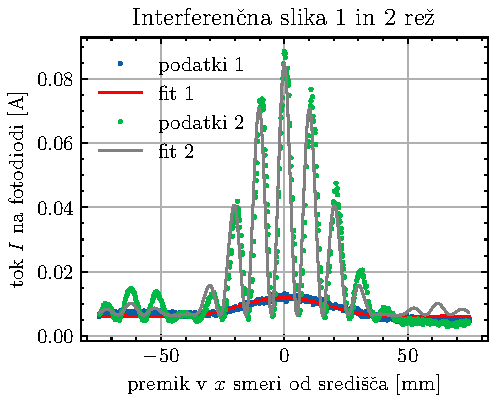
\includegraphics[width=8cm]{uklon12.pdf}
    \caption{Uklonska slika na eni in dveh režah}
    \label{1}
\end{center}
\end{figure}
\begin{figure}[ht]
\begin{center}
    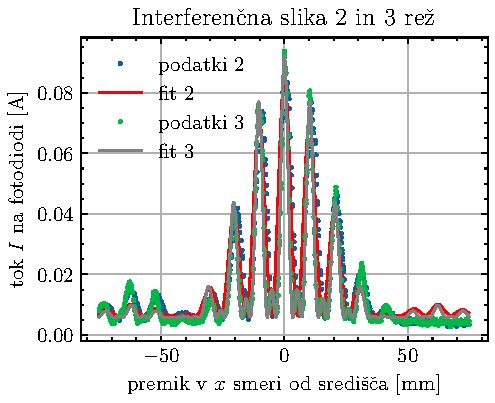
\includegraphics[width=8cm]{uklon23.pdf}
    \caption{Uklonska slika na dveh in treh režah}
    \label{2}
\end{center}
\end{figure}
\begin{figure}[ht]
\begin{center}
    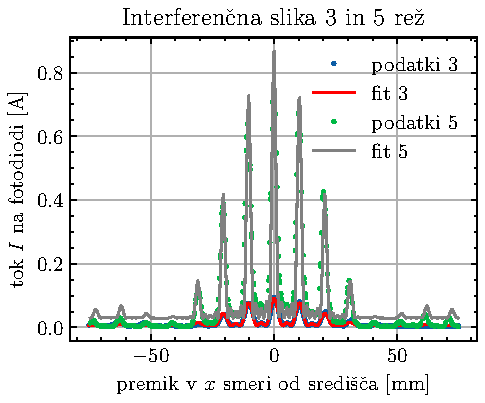
\includegraphics[width=8cm]{uklon35.pdf}
    \caption{Uklonska slika na treh in petih režah}
    \label{3}
\end{center}
\end{figure}
\begin{figure}[ht]
\begin{center}
    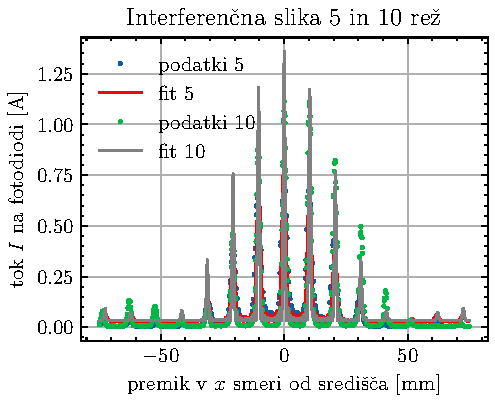
\includegraphics[width=8cm]{uklon510.pdf}
    \caption{Uklonska slika na petih in desetih režah}
    \label{5}
\end{center}
\end{figure}

\begin{table}[!ht]
\centering
\begin{tabular}{c||c|c|c}
    $n$     & $I_0$ & $a$            & $b$              \\\hline \hline
    1       & 0.006 & 0.022          & 0.097            \\
    2       & 0.020 & 0.023          & 0.096            \\
    3       & 0.01  & 0.023          & 0.097            \\
    5       & 0.034 & 0.023          & 0.097            \\
    10      & 0.013 & 0.020          & 0.097            \\\hline
    average & /     & $0.022\pm 0.002$ & $0.097\pm 0.001$
\end{tabular}
\caption{Parametri fita}
\label{params}
\end{table}

\newpage
Parametra $a$ in $b$ sta povezana z debelino rež in razdaljo med njimi, tako da sedaj lahko določimo ta dva podatka:

\begin{equation*}
    D = a \lambda s = (31.1\pm 0.6)\mu m
\end{equation*}
\begin{equation*}
    d = b \lambda s = (144\pm 2)\mu m
\end{equation*}

\noindent Na žalost nam ni uspelo primerjati relativnih intenzitet smiselno, razlog za kar mislim, da je dejstvo, da smo morali laser komstantno nekoliko premikati, da je slika ostala vodoravna, tako da posledično delež intenzitete, ki ga je dioda zaznala ni bil konstanten. V teoriji bi morala biti relativna intenziteta sorazmerna s kvadratom števila rež.

V drugem delu naloge smo merili debelino okrogle odprtine, tako da smo opazovali interferenčno sliko, ki so jo zaznamovale Fresnelove cone. Merili smo pri katerih odmikih reže smo opazovali minimume in kje maksimume. Najprej smo morali izmeriti ničto razdaljo med laserjem in režo $d_o = (20.5\pm o.1)\ cm$, med odprtino in sliko pa $d_1 = (179.3\pm 0.3)\ cm$. Na merilu na tej točki izmerimo $x_0 = (19.2\pm 0.1)\ cm$. Minimume in maksimume predstavimo v tabeli \ref{fresny} skupaj s preračunanimi vrednostmi $z_p$; razdalja od gorišča leče do odprtine in $z_0$; razdalja od odprtine do slike ter $1/\zeta = 1/z_0 + 1/z_p$.

\begin{table}[!ht]
\centering
\begin{tabular}{c|c|c|c|c}
    tip & $x\ (\pm 0.2\ cm) $ & $z_p\  (\pm 0.3\ cm) $ & $z_o\  (\pm 0.2\ cm) $ & $1/\zeta$ [$cm^{-1}$]\\\hline
    min & $15.7$ & $17.0$ & $182.8$ & $0.064\pm 0.001$ \\
    max & $14.4$ & $15.7$ & $184.1$ & $0.069\pm 0.001$ \\
    min & $12.0$ & $13.3$ & $186.5$ & $0.080\pm 0.002$ \\
    max & $10.2$ & $11.5$ & $188.3$ & $0.092\pm 0.002$ \\
\end{tabular}
\caption{Tabela minimumov in maksimumov}
\label{fresny}
\end{table}

\noindent Za tem lahko grafiramo odvisnost $1/\zeta$ od indeksa Fresnelove cone. To odvisnost prikažemo na grafu \ref{lin}:

\begin{figure}[ht]
\begin{center}
    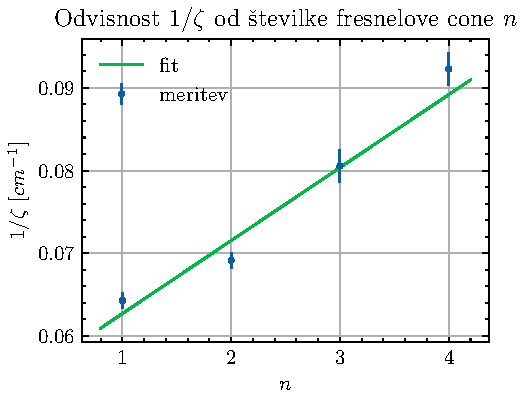
\includegraphics[width=8cm]{lin.pdf}
    \caption{odvisnost $1/\zeta$ od indeksa Fresnelove cone}
    \label{lin}
\end{center}
\end{figure}
Na istem grafu je narisan tudi najboljši linearen fit premice $y=ax+b$; kjer sta izmerjena parametra:
\begin{equation*}
    a = (9\pm 1)10^{-3} cm^{-1}, b = (0.05\pm 0.01) cm^-1
\end{equation*}
Iz tega izračunamo $n_0=b/a\approx 6$ in pomambneje:
\begin{equation*}
    D = 2\sqrt{\frac{\lambda}{a}} = (1.7\pm 0.1) mm
\end{equation*}

\end{document}